\newpage
\subsection{2-String Kite}
Die Technik \textit{2-String-Kite} wird auch Paierdrache genannt, was sich, wie beim Wolkenkratzer, aus der Anordnung der Zahlen ableitet. Auch hier wird nur eine einzige Ziffer betrachtet. Gesucht werden eine Zeile und eine Spalte, die nur noch zwei Kandidaten der betrachteten Ziffer enthalten, so dass ein Kandidat der Spalte und ein Kandidat der Zeile im selben Block liegen. Die Zeile und die Spalte nennt man die \textit{Schnüre} des Drachens. Die Enden der Schnüre liegen im gleichen Block, die Position des Anfangs ist relevant für das Löschen des Kandidaten. Gelöscht werden kann nämlich der Kandidat in der Zelle, die von beiden Anfängen der Schnüre ausgeschlossen wird. Das kommt zustande, da die betrachtete Ziffer in jedem Fall am Anfang einer der beiden Schnüre stehen muss.

\begin{figure}[h]
\begin{center}
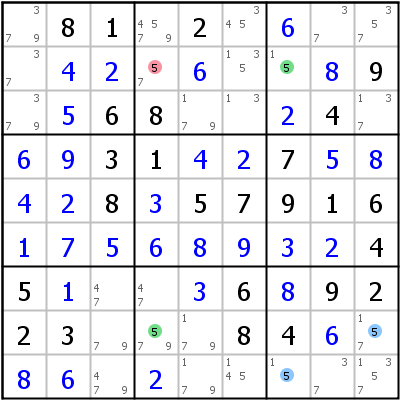
\includegraphics{./img/2stringkite.png}
\caption{2-String-Kite}
\end{center}
\end{figure}

\textbf{Abbildung 3.10} zeigt einen \textit{2-String-Kite}. Betrachtet wird die Ziffer 5, Zeile 8 und Spalte 7 fungieren als Schnüre des Drachen. In z2s7 betrachten wir zwei Fälle: Entweder die Ziffer 5 steht dort oder sie steht dort nicht. Für den ersten Fall gilt, dass dann die rot markierte Ziffer in z2s4 ausgeschlossen ist. Der zweite Fall ist etwas komplizierter. Wenn die Ziffer 5 nicht in z2s7 steht, dann muss sie an der einzig anderen möglichen Position der Spalte stehen, nämlich in z9s7. Daher kann sie nicht in z8s9 stehen, da diese Felder im selben Block liegen. Da in Zeile 8 auch nur noch zwei Kandidaten für die Ziffer 5 übrig waren, muss sie in z8s4 stehen, wi sie z2s4 ausschließt. In jedem der Fälle kann also die Ziffer 5 nicht in z2s4 stehen und daher kann sie dort gelöscht werden.